\documentclass[10pt,journal]{IEEEtran}
\usepackage{graphicx}
\usepackage{amsmath,amssymb}
\usepackage{url}
\usepackage[hidelinks]{hyperref}

\begin{document}

\title{Epoch-Fenced Safety Rule Enforcement in ROS 2 Robot Fleets:
Design, Fault Injection, and Recovery}

\author{} % double-anonymous initial submission: no author block

\maketitle

\begin{abstract}
Fleet-wide safety-rule changes, e.g.\ newly declared keep-out zones,
reach robots at different times under partitions, crashes, and loss.
A robot that misses the update can keep executing obsolete rules with
no bound: we exhibit this stale-rule window against broadcast and
plain two-phase commit (2PC), in a checker and in ROS 2, with stale
execution reaching 12.7~s and a 40.4~s drive-through in Gazebo.
This paper presents the design, fault-injection evaluation, and
recovery behavior of a ROS 2 enforcement stack that combines
long-established mechanisms---versioned rule snapshots, leases,
fencing generations, 2PC structure, write-ahead logging, retries
with fresh attempt identity, and pull reconciliation---with
per-command motion authorization at the last software boundary and a
per-decision audit ledger. We claim no new distributed mechanism; a
careful composite baseline using the same parts was never implemented
and we claim no superiority over it. Measured on a frozen fault
battery (480-run matrix, 5-robot injection, 20-agent eventual-heal
with 100/100 commits, Gazebo witnesses), obsolete-rule motion
authorization ends within a 1300~ms engineering budget (worst
observed cell 552~ms), partitioned and restarted robots hold motion
until reconciled, and removed mechanisms reproduce the failures as
positive controls (up to 7792.2~ms stale). We keep three concepts
separate throughout: bounded stale-motion \emph{authorization},
physical motion \emph{stopping}, and actual \emph{compliance} with
newly activated constraints---only the first is bounded here. All
experiments use lightweight ROS 2 processes on a single host plus
Gazebo physics; there is no hardware validation.
\end{abstract}

\begin{IEEEkeywords}
Robot fleet safety; safety-rule updates; leases and fencing;
fault injection; runtime assurance; ROS 2.
\end{IEEEkeywords}

\section{Introduction}
\label{sec:intro}

Consider a fleet of mobile robots sharing a set of hard safety rules,
for example keep-out polygons published by a facility operator. When
a rule changes, the update must reach every robot; the network between
the fleet coordinator and the robots is hostile in routine ways:
partitions, crashes, restarts, message loss, duplication, delay, and
reordering. The failure that motivates this work is simple and, in
our measurements, severe: a robot that misses a rule update keeps
executing the obsolete rule set with \emph{no bound}. In our ROS 2
fault-injection battery, plain 2PC exhibits stale execution up to
12.7~s on single faults, and in a Gazebo witness a partitioned robot
under plain 2PC drives the stale nominal route straight through a
newly declared keep-out zone for 40.4~s.

This raises a practical systems research question rather than an
algorithmic one: \emph{can the combination of versioned snapshots,
leases, fencing, and reconciliation be assembled into a ROS 2 fleet
so that obsolete-rule motion authorization provably ends within a
stated budget after each superseding commit, partitioned and
restarted robots cannot act until reconciled, and every authorization
decision is auditable---and what breaks, exactly, when any one piece
is removed?} The mechanisms involved are established distributed
systems practice; our contribution is their B3-honest assembly (we
define the careful composite baseline in Section~II and claim nothing
over it), its measurement under a frozen fault battery, and the
retained negative results along the way.

Concretely, this paper contributes: (C1) a ROS 2 implementation of
epoch- and hash-tagged hard-rule snapshots, lease-bound rule
currency, fencing generations, a reachable-unanimity transaction
path with generation-scoped attempts and durable commit order, plus a
conjunctive per-command motion gate with a per-decision audit ledger;
(C2) a reproducible fault-injection and evidence-validation
methodology covering communication faults, crashes, restarts,
recovery, and failed rounds, with a validity ledger that voids
workloads rather than spinning them; (C3) an empirical
characterization of stale-motion authorization and its disciplined
separation from physical stopping and from rule compliance. We
explicitly disclaim fundamental novelty in 2PC, fencing, leases,
write-ahead logging, message retries, and reconciliation.

The remainder reports design (III), properties with explicit
assumptions (IV), setup (V), results with failure analysis (VI),
and limitations (VII).

\section{Related Work}
\label{sec:related}

\emph{The strong composite baseline (B3).} A careful design combining
2PC with local lease expiry, actuation-side fencing, epoch
reconciliation, and fail-safe HOLD reproduces, on paper, every safety
invariant in Section~IV using the same state our system holds. B3 was
never implemented or evaluated here, so no comparison against it is
reported; it is the lens through which our mechanism claims must be
read, and it is why this paper claims an assembly and its
measurement, not a protocol. The test is stated plainly so reviewers
can apply it: exhibit a trace in which a carefully built B3 violates
an invariant our system holds, and the equivalence account fails;
none is known, and the counterexample suites in Section~VI target
plain 2PC and broadcast only.

\emph{Leases and fencing.} Chubby's lock service~\cite{burrows2006chubby}
combines session leases with KeepAlive renewal and sequencers---opaque
lock-plus-generation strings that recipient servers must check before
acting---which is the direct lineage of our fence generation and
highest-seen rejection. The fencing-token formulation, that safety
against paused holders must be enforced at the resource rather than
by timing assumptions, is standard~\cite{kleppmann2016locking}.

\emph{Versioned updates without partitions.} Consistent network
updates~\cite{reitblatt2012abstractions} and timed consistent
updates~\cite{mizrahi2015timed} version configurations and prove
per-packet consistency, but assume a connected controller (and, for
the latter, synchronized clocks) and stateless forwarding. Our design
refuses both assumptions: safety here rests on per-robot local
monotonic clocks for lease expiry, with no cross-node synchronization
required, and on stateful per-robot authorization.

\emph{Supervision without distribution.} Runtime assurance and the
Simplex architecture~\cite{seto1998simplex,sha2001simplicity},
standardized for aircraft in ASTM F3269~\cite{astmF3269}, place a
monitor and a recovery function at the control boundary of a single
system. Our motion gate follows that shape (gate plus HOLD-as-recovery)
but adds the distributed half those works omit: versioned snapshots,
leases, fencing across a fleet, and reconciliation.

\emph{Fleet rule rollout without guarantees.} Open-RMF closes
navigation-graph lanes at runtime and replans affected robots, but
offers explicitly no strong guarantees about effectiveness, and a
partitioned robot keeps its old graph unboundedly~\cite{openrmf2021laneclosure}.
Static command authorization exists in SROS 2 over DDS
Security~\cite{sros2accesscontrol,ros2ddsssecurity}: signed policies
control who may publish what, but policies carry no epoch or lease
currency and cannot express ``this command is stale.'' A policy can
deny a topic to a node; it cannot admit a command only while its
rule version is current, which is the entire temporal content of our
gate. Single-vehicle geofence monitoring with mitigation
ladders~\cite{torens2020geofencing} contains one vehicle; fleet-wide
content updates under partition are outside its model, and none of
its buffers bound cross-version staleness.

\emph{2026 execution-finality disclosures.} Two individual
Informational Internet-Drafts (unreviewed, not IETF-adopted, not
peer-reviewed) disclose adjacent ideas for single platforms: per-act
execution finality at a Finality Sink with monotonic authority
epochs and HOLD-state composites for multi-aircraft
acts~\cite{das2026actfinality}, and an actuation-bound invariant over
exact command, actuator, current authority, freshness, and
non-bypassable path~\cite{das2026actuationbound}. They cover the
gate half of our design space for single platforms, without fleet
commit semantics; we cite them as disclosures with correct status,
not as standards.

\section{System Design and Motion Authorization}
\label{sec:design}

Three single-purpose process roles per fleet (Fig.~1) communicate over
fixed ROS 2 topics carrying JSON string messages~\cite{macenski2022ros2}:
a coordinator (propose/decide/COMMIT/RENEW, one OS process), one rule
agent per robot (adopt/lease/reconcile state plus a crash-safe state
file), and one MotionFence per robot (the last software boundary
before motion release). A durable write-ahead log (WAL) on the
coordinator and a per-decision fence ledger on each robot (fsync'd
before any ACCEPT is evidenced) make every safety-relevant step
auditable.

\begin{figure}[t]
\centering
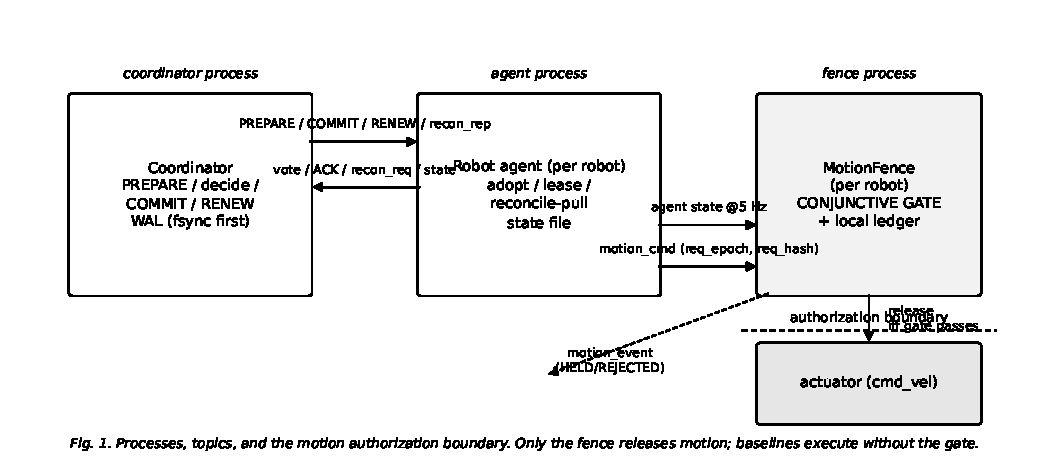
\includegraphics[width=\columnwidth]{figures/fig1_architecture.pdf}
\label{fig:arch}
\end{figure}

\emph{Rule snapshots.} Each epoch $e$ carries a hard-rule payload
(keep-out polygons) with snapshot hash $h(e)$ (SHA-256 over canonical
JSON). Every PREPARE/COMMIT carries $(e,h(e),\text{fence},\text{rules})$;
agents verify the hash before voting READY, before applying a COMMIT,
and before applying a reconcile reply. Equal epochs therefore imply
equal rule sets wherever adoption is verified.

\emph{Commit path.} The coordinator proposes epoch $e{+}1$ with one
PREPARE per attempt; attempts carry identity
$\mathit{tx}(e,h,g)$ with a generation $g$ that increments past
aborted generations on every re-proposal. Robots vote READY/REJECT
once per transaction (duplicate PREPAREs are recognized and emit
nothing further; older generations are ignored; newer ones supersede).
The coordinator commits iff every \emph{observed-reachable} robot
(state seen within 2000~ms) voted READY; a robot silent beyond that
window is excluded from the threshold and its safety is carried
entirely by lease expiry (leases are 1000~ms, so excluded robots are
already holding). Generations keep liveness moving without touching
that rule: a re-proposed epoch starts a fresh generation that skips
aborted ones, agents supersede older generations of the same epoch,
duplicate PREPAREs are recognized silently, ABORT clears only its own
transaction, and an already-applied COMMIT replays as an idempotent
no-op plus acknowledgment---so retries can neither roll back nor
double-apply. Commit linearizes at the WAL append, which precedes
the COMMIT publish; ABORT records distinguish timeout from reject and
are never resurrected. On restart the coordinator re-fences
($\text{fence}+1$), replays the durable COMMIT exactly once, and
resumes pending epoch $e{+}1$; missed-COMMIT catch-up is pull-side
(reconcile requests), never a redrive loop.

\emph{Contact sync (adopt-only-current).} A COMMIT grants a 1000~ms
lease. Agents extend their lease deadline only on adopted-currency
contact: same-epoch RENEW, COMMIT, or reconcile reply. A newer-epoch
RENEW triggers a reconcile pull without adoption; an obsolete-epoch
RENEW is ignored. The naive alternative---extending the lease on any
coordinator contact---is exactly the renewal bug our A3 control
reproduces (Section~VI).

\emph{Motion gate.} Every motion command carries
$(\text{required\_epoch},\text{required\_hash})$. The fence releases
it iff all hold at the decision instant: required epoch equals the
agent's committed epoch; hashes match; local time is within the lease
deadline; the agent is reconciled; the agent is not holding. Otherwise
the command is REJECTED (epoch/hash mismatch) or HELD (lease expired,
unreconciled, agent holding) with a latched reason, and a safe-stop
event is emitted. Baselines execute every command (logged ``no-gate'')
so matrices stay comparable; the missing gate is the defect under
test. Restarted agents load durable (epoch, hash, fence seen) and
start UNRECONCILED, so no motion is possible before reconciliation.
Reconciliation itself is pull-side and boring by design: an
unreconciled agent re-requests roughly every second, the coordinator
answers with its current durable epoch, and the reply installs
(epoch, hash), ratchets the fence seen, extends the lease, and clears
holding---or is ignored on any hash or fence mismatch. The holding
flag is recomputed at 5~Hz from reconciled status and lease liveness,
so either expiry path converges to HELD verdicts without any
coordinator interaction, which is what makes the fail-safe default
hold under total coordinator loss.

\emph{Budget.} Stale authorization after a superseding commit is
bounded by construction: no adoption and no renewal at obsolete
currency can occur past the commit, so the covering lease was granted
no later than commit time. With the frozen budgets---1000~ms lease,
50~ms fence-scheduling guard, 250~ms in-flight drain---the bound is
$B_{\text{real}}=1300$~ms (Fig.~2). These are stated timing
assumptions (Section~IV), not measurements.

\begin{figure}[t]
\centering
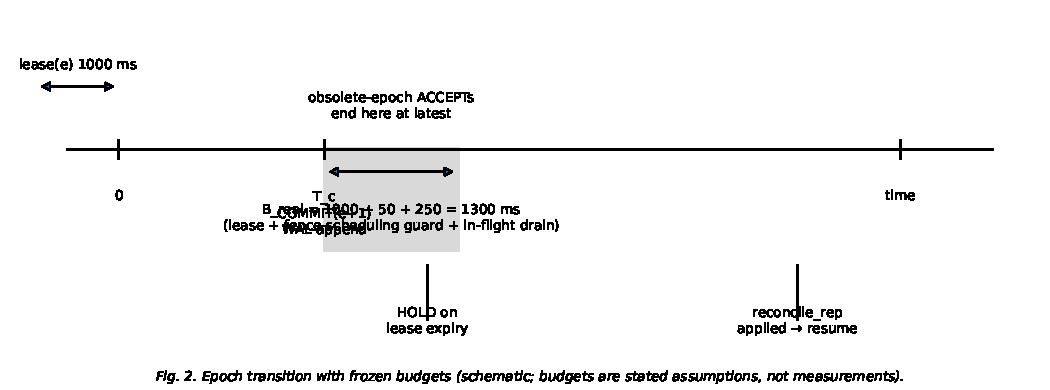
\includegraphics[width=\columnwidth]{figures/fig2_epoch_transition.pdf}
\label{fig:epoch}
\end{figure}

\section{Safety Properties and Assumptions}
\label{sec:props}

Checked properties I1--I7: committed epochs never decrease (I1);
equal epochs imply equal hashes where adoption is verified (I2);
executed motion matches local committed epoch (I3); out-of-contact
past lease implies no motion (I4); stale-epoch execution ends within
the bound after a fleet commit (I5); restart restores nothing
actionable without reconcile (I6); reconnect reconciles before motion
resumes (I7). Status is explicitly bounded: exhaustive checking at
$n{=}3$ within documented horizons plus a small TLA+ gate model, and
ROS-level measurement elsewhere; the unbounded proof is future work
and is not claimed. I2 is vacuous in the fault model without content
mutation and is covered in ROS by payload-mutation tests instead.

Assumptions, all load-bearing, are summarized in Table~I: local
monotonic clocks (no cross-node sync needed for safety); fence
scheduling within 50~ms; in-flight command drain within 250~ms; an
honest (non-equivocating) coordinator; filesystem integrity for the
WAL and state files; code-path restart behavior; no fence bypass;
commands actually routed through the fence. Removing clock
monotonicity refutes the bound (the standard clock-jump class);
starving the fence or the actuator drain opens it; equivocation and
crash-during-write are outside the tested model. Single-host
experiments exercise none of the cross-machine clock behavior;
per-robot locality of lease expiry is what keeps the safety case
intact there.

\begin{table}[t]
\caption{Load-bearing assumptions (all required for the bound).}
\label{tab:assump}
\centering
\footnotesize
\begin{tabular}{ll}
\hline
ID & Assumption (removal consequence) \\
\hline
A1 & Local monotonic clocks; clock jump refutes bound \\
A2 & Fence decides within 50~ms; starvation opens bound \\
A3 & In-flight drain within 250~ms; else motion outlives grant \\
A4 & Honest coordinator; equivocation outside model \\
A5 & WAL/state-file integrity; crash-during-write untested \\
A6 & Restart follows code path (UNRECONCILED / fence+1) \\
A7 & No fence bypass (controls A1/A2 show the open gate) \\
A8 & Commands routed through fence (deployment wiring) \\
\hline
\end{tabular}
\end{table}

The trichotomy used throughout: (A) \emph{stale-motion
authorization} is what $B_{\text{real}}$ bounds; (B) \emph{physical
motion stopping} adds actuator and vehicle dynamics and is only ever
measured, never bounded here; (C) \emph{compliance with newly
activated constraints} additionally requires egress geometry and
time, and is never claimed as immediate. A robot inside a new
keep-out zone at commit time needs egress time no authorization bound
can supply.

\section{Experimental Setup}
\label{sec:setup}

\emph{Harness (with one disclosed deviation).} All impairments run in
a deterministic in-node shim (drop/duplicate/delay/mutate by
byte-replayable JSON schedules) instead of netns/tc; ROS 2, DDS
discovery, crashes (process kill), and clocks are real. The closed
fault list is applied identically to every protocol: message delay,
drop, duplicate, reorder, robot crash/restart, coordinator
crash/restart, partition and heal, late commit, stale command, and
reconnect. This was a frozen preregistered deviation, symmetric
across protocols, and it is why our middleware timing (including a
41-node discovery storm in the scale runs) is real while our links
are not.

\emph{Schedules and metrics.} A 16-fault deterministic matrix
(F0--F15, 30 repetitions each, 480 runs) plus 5-robot systematic and
combined schedules; eventual-heal (W-HEAL) and sustained-loss
(W-SUSTAINED) workloads with a machine-checked global-stabilization
time gate that voids liveness readings from non-healing runs; three
Gazebo witness scenarios with a blessed harness. Metrics:
contradictory authorizations (epoch mismatch + invalid lease +
unreconciled, must be 0), worst stale authorization vs $B_{\text{real}}$,
heal-to-commit latency, and ledger-join audits (every ACCEPT joined
against epoch/hash equality, live lease, reconciled-and-not-holding;
missing ledgers mean evidence-incomplete, never pass). A
machine-checked global-stabilization-time gate marks each record
workload-valid only if all faults expire inside the run; records that
end before stabilization are excluded from every liveness reading
automatically, with the reason recorded---this is what voids the two
early heal-workload rounds (Section~VI) instead of letting permanently
stacking loss pose as a healing workload.

\emph{Scale and physics disclosure.} Fleet-scale runs use lightweight
ROS 2 processes (1 coordinator + 20 agents + 20 fences) on a single
host---not physical robots. Physics appears only in the Gazebo
witnesses~\cite{koenig2004gazebo}. Vote timeout is 1500~ms (harness
stability, not a gate); control topics use BEST\_EFFORT depth
$\max(32,2N{+}8)$.

\section{Results and Failure Analysis}
\label{sec:results}

\emph{Counterexamples (T0).} Nine systematic schedules plus 400
randomized fault schedules per protocol at $n{=}3$ exhibit the
plain-2PC stale-rule window (partitioned robot executing obsolete
rules unboundedly), a late-COMMIT rollback violating monotonicity,
and superseded-epoch execution after restart; broadcast adds hash and
reconcile violations. The same battery is clean under the fence/lease
design within its bounds (worst 1 tick vs bound 5; 8472-state TLC
gate model clean). Table~II collects the ROS-level campaigns.

\begin{table}[t]
\caption{Frozen ROS evidence at a glance (all single-host).}
\label{tab:evidence}
\centering
\footnotesize
\begin{tabular}{lccc}
\hline
Campaign & Scale & Worst stale & Ledger join \\
\hline
Matrix F0--F15 & 3 robots $\times$30 & 153.8~ms & 480/480 clean \\
30$\times$ repeat & 3 robots $\times$30 & 181.3~ms & clean \\
5-robot + I2 & 5 robots, 11 sched & 163.1~ms & clean \\
W-HEAL & 20 agents, 100 upd. & 263.2~ms & 6059 ACCEPTs clean \\
W-SUSTAINED & permanent loss & 150.0~ms & 1632 ACCEPTs clean \\
M matrix & 20 agents, 480 runs & 552~ms cell & 480/480 clean \\
N restart & 5 robots, 11 sched & 184~ms & clean \\
Q witness & Gazebo $\times$3 & 58--130~ms & 3/3 clean \\
A3 control & renewal bug & 7792.2~ms & bug reproduced \\
\hline
\end{tabular}
\end{table}

\emph{Fault matrix (480 runs).} All 16 EFRS cells show zero
contradictory authorizations and zero rollbacks, worst stale
authorization 153.8~ms; the 30$\times$ campaign peaks at 181.3~ms
(7$\times$ under budget). Baselines reproduce the defect on the same
faults: broadcast 7.7--12.5~s stale, 2PC 7.9--12.7~s, plus 90
rollbacks on one 2PC cell. Five-robot schedules peak at 163.1~ms with
zero violations; integrity tests reject mutated payloads (341/230
fence rejections) while legitimate epochs commit unaffected.

\begin{figure}[t]
\centering
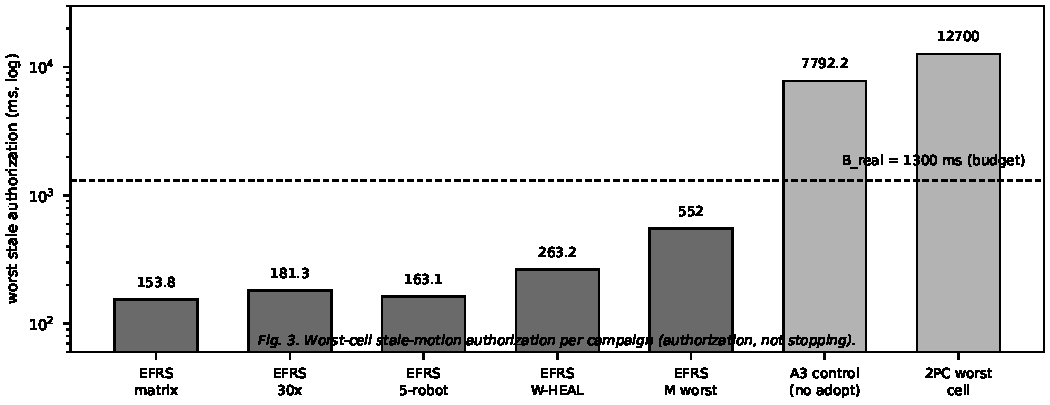
\includegraphics[width=\columnwidth]{figures/fig3_stale_results.pdf}
\label{fig:stale}
\end{figure}

\emph{Healing and sustained loss.} W-HEAL commits 100/100 distinct
epochs (100 issued; 3 aborts recovered by fresh-generation
re-attempts, every committed update within 2 attempts; 106 PREPARE
broadcasts total, i.e.\ about 1.06 per committed update, plus 100
COMMITs and 2036 received votes with no redrives or retransmits).
Heal-to-commit peaks at 2.06~s (median 1.22~s) against a 10~s bound;
worst stale authorization is 263.2~ms; 20/20 ledgers join clean
(31{,}989 rows, 6{,}059 ACCEPTs). W-SUSTAINED under permanent loss
commits 2/100 (descriptive only) with 51 aborts, worst stale
150.0~ms, and ledgers clean---fail-safe HOLDs under degradation, not
progress. The corrected 20-agent W-HEAL matrix round is 480/480
ledger-clean with cell maxima 0--552~ms.

\emph{Restarts.} Coordinator-plus-robot restart replays the durable
epoch exactly once and commits the next epoch 0.18~s post-restart
with zero rollbacks and a clean ledger; 8/11 five-robot fault/restart
schedules commit fully with zero violations.

\emph{Physical witnesses.} Three Gazebo scenarios (Fig.~4, T1 origins
$t{=}2/5/25$~s with T13a bounds annotated) show the
same shape: R3 partitioned for 23~s holds motion under 112--113
lease-expired verdicts, heals, reconciles to epoch~1, egresses south
within 3.1~s, detours, and resumes to goal; runner-measured stale
authorization stays 58--130~ms and all three fence ledgers join clean.
The same scenario under plain 2PC never commits and drives stale
through the zone. Egress latency is reported, not bounded: robots
inside the zone at commit time need geometric egress no authorization
bound can supply.

\emph{Positive controls.} Removing the fence yields 31 unauthorized
accepts (A1) and removing leases 32 (A2). Restoring naive contact
renewal (extend-without-adopt) reproduces 7830.8~ms stale in T1 and
7792.2~ms in the corrected rerun, with the fleet epoch stuck while
214 unadopted renewals arrive---the exact bug the adopt-only-current
rule excludes, and evidence the stale metric fires when mechanisms are
removed.

\emph{Negative findings (retained).} The original 20-robot scale run
committed 0/100: only 13/20 READY votes arrived inside the single-shot
1500~ms window, the coordinator had no abort/retry path, its
\texttt{prepared} flag stayed set, and all 99 subsequent proposes were
rejected silently over 265~s---while 237 correct lease-HOLDs kept
stale motion at zero, which is fail-safe behavior, not success. The
first two heal-workload rounds ran under
permanently stacking loss because a runner bug never expired
\texttt{loss\_random} faults, voiding their liveness readings (safety
readings stand as sustained-loss stress); the transport comparison
built on those rounds is void for causal inference and the
congestion hypothesis is downgraded to an open secondary question;
one coordinator-restart execution preceded its amendment commit
(disclosed order deviation with post-hoc code-identity proof); ACK
counting, RTPS meta-traffic, and some live QoS captures are missing
instrumentation, carried as gaps. Plain 2PC is the weaker baseline
on purpose: it exhibits the defect class. The careful B3 composite
was never implemented, so no quantitative language in this paper
implies any measured advantage over it.

\begin{figure}[t]
\centering
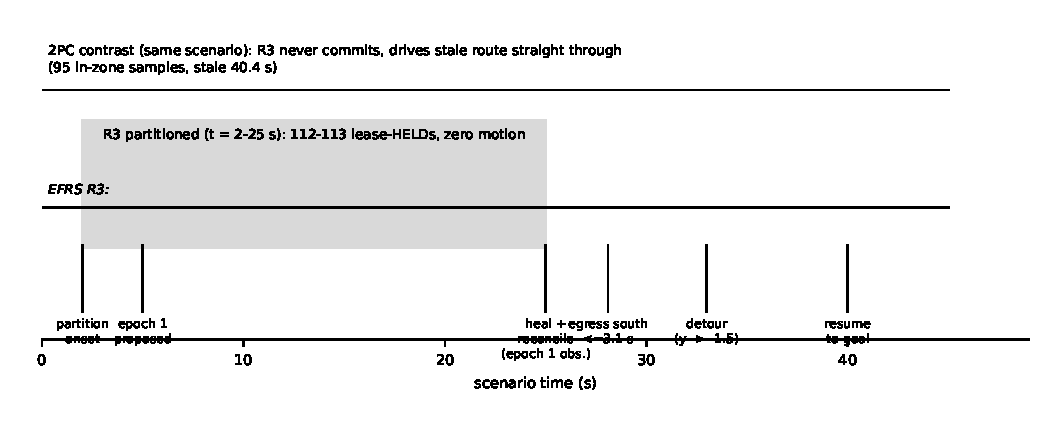
\includegraphics[width=\columnwidth]{figures/fig4_witness_timeline.pdf}
\label{fig:witness}
\end{figure}

\section{Limitations and Conclusion}
\label{sec:limit}

Limits are stated, not buried. No unbounded or arbitrary-$n$ proof
exists, and the small-instance checks do not generalize by
themselves. Multi-machine clock behavior is untested (safety needs
only per-robot local monotonicity, but every timing measurement
assumes it). Guard and drain budgets are measured consistent but
unstressed near the bound, so $B_{\text{real}}$ is validated with
margin, not probed to failure. Physics is Gazebo-only with no
hardware validation: actuator latency, radio behavior, and sensing
are all absent, and the witness egress times describe one scenario
family. Permanent-loss tails are inconclusive for liveness---repair
is demonstrated for healing workloads only. Transport findings are
void, congestion reasoning is downgraded, and several instrumentation
gaps (ACK counts, RTPS meta-traffic, some live QoS captures) are
carried openly. B3 was never built, so no superiority over it is
claimed or measurable here, and any reviewer-supplied B3 that
reproduces our invariants on paper is consistent with, not fatal to,
this paper's assembly-and-measurement claim. Sensor-corruption
(SCOPE) results from a sibling project are quarantined out of this
account. Six pages cannot carry the full fault battery: the frozen
schedules, ledgers, and analysis scripts are released as artifacts
for independent audit, and all page content here is self-contained.

In conclusion, established mechanisms---epochs, hashes, leases,
fencing generations, 2PC structure, durable logging, fresh-identity
retries, pull reconciliation---can be assembled into a ROS 2 fleet
whose obsolete-rule motion authorization ends within a stated,
measured budget, whose partitioned and restarted members hold motion
until reconciled, and whose every authorization decision is
auditable. The measurement, the retained failures, and the
authorization/stopping/compliance distinction are the contribution;
no new distributed mechanism is claimed.

\bibliographystyle{IEEEtran}
\bibliography{references}

\end{document}